\footnotesize
\begin{tikzpicture}
\begin{scope}[xshift=4cm]
\draw[pattern=north west lines](0,0)rectangle(3,.3);
\draw[pattern=north west lines](0,-4)rectangle(3,-4.3);
\draw[pattern=north west lines](1.35,0)rectangle(1.65,-4);
\draw[draw=cc0066,line width=.8mm,fill=cc0066!20](.4,0)rectangle(1.35,-4);
\draw[draw=cc0066,line width=.8mm,fill=cc0066!20](2.6,0)rectangle(1.65,-4);
\node at(1.5,-5.5)[align=center]{both sided\\full height\\stiffener};
\end{scope}
\begin{scope}[xshift=9cm]
\draw[pattern=north west lines](0,0)rectangle(3,.3)node[below=4mm]{in compression};
\draw[pattern=north west lines](0,-4)rectangle(3,-4.3)node[above=4mm]{in tension};
\draw[pattern=north west lines](1.35,0)rectangle(1.65,-4);
\draw[draw=cc0066,line width=.8mm,fill=cc0066!20](.4,0)rectangle(1.35,-3);
\node at(1.5,-5.5)[align=center]{single sided\\partial height stiffener\\to avoid fatigure fracture};
\end{scope}
\node at(0,-3){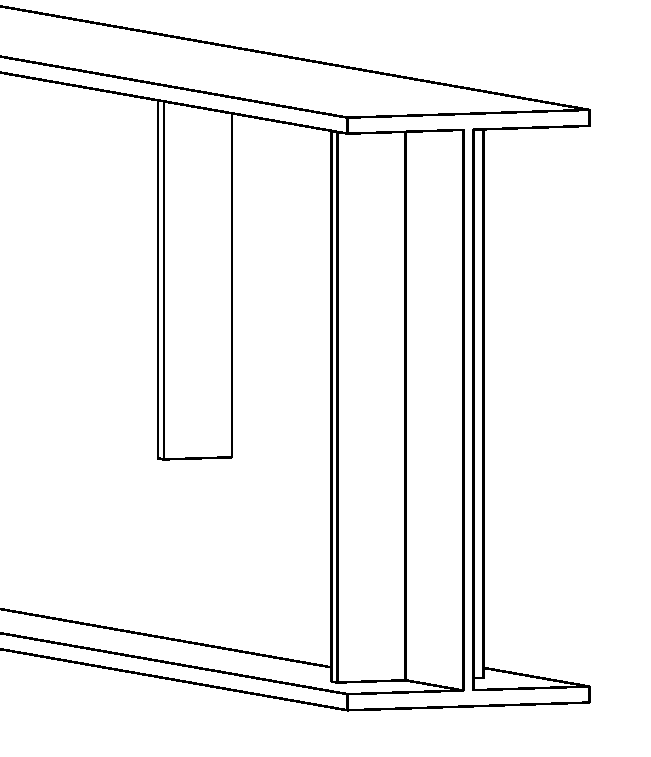
\includegraphics[height=6cm]{PIC/CH05/STIFFENER}};
\end{tikzpicture}